
%% bare_jrnl_comsoc.tex
%% V1.4b
%% 2015/08/26
%% by Michael Shell
%% see http://www.michaelshell.org/
%% for current contact information.
%%
%% This is a skeleton file demonstrating the use of IEEEtran.cls
%% (requires IEEEtran.cls version 1.8b or later) with an IEEE
%% Communications Society journal paper.
%%
%% Support sites:
%% http://www.michaelshell.org/tex/ieeetran/
%% http://www.ctan.org/pkg/ieeetran
%% and
%% http://www.ieee.org/

%%*************************************************************************
%% Legal Notice:
%% This code is offered as-is without any warranty either expressed or
%% implied; without even the implied warranty of MERCHANTABILITY or
%% FITNESS FOR A PARTICULAR PURPOSE! 
%% User assumes all risk.
%% In no event shall the IEEE or any contributor to this code be liable for
%% any damages or losses, including, but not limited to, incidental,
%% consequential, or any other damages, resulting from the use or misuse
%% of any information contained here.
%%
%% All comments are the opinions of their respective authors and are not
%% necessarily endorsed by the IEEE.
%%
%% This work is distributed under the LaTeX Project Public License (LPPL)
%% ( http://www.latex-project.org/ ) version 1.3, and may be freely used,
%% distributed and modified. A copy of the LPPL, version 1.3, is included
%% in the base LaTeX documentation of all distributions of LaTeX released
%% 2003/12/01 or later.
%% Retain all contribution notices and credits.
%% ** Modified files should be clearly indicated as such, including  **
%% ** renaming them and changing author support contact information. **
%%*************************************************************************


% *** Authors should verify (and, if needed, correct) their LaTeX system  ***
% *** with the testflow diagnostic prior to trusting their LaTeX platform ***
% *** with production work. The IEEE's font choices and paper sizes can   ***
% *** trigger bugs that do not appear when using other class files.       ***                          ***
% The testflow support page is at:
% http://www.michaelshell.org/tex/testflow/



\documentclass[journal,comsoc]{IEEEtran}
%
% If IEEEtran.cls has not been installed into the LaTeX system files,
% manually specify the path to it like:
% \documentclass[journal,comsoc]{../sty/IEEEtran}


\usepackage[T1]{fontenc}% optional T1 font encoding


% Some very useful LaTeX packages include:
% (uncomment the ones you want to load)


% *** MISC UTILITY PACKAGES ***
%
%\usepackage{ifpdf}
% Heiko Oberdiek's ifpdf.sty is very useful if you need conditional
% compilation based on whether the output is pdf or dvi.
% usage:
% \ifpdf
%   % pdf code
% \else
%   % dvi code
% \fi
% The latest version of ifpdf.sty can be obtained from:
% http://www.ctan.org/pkg/ifpdf
% Also, note that IEEEtran.cls V1.7 and later provides a builtin
% \ifCLASSINFOpdf conditional that works the same way.
% When switching from latex to pdflatex and vice-versa, the compiler may
% have to be run twice to clear warning/error messages.






% *** CITATION PACKAGES ***
%
%\usepackage{cite}
% cite.sty was written by Donald Arseneau
% V1.6 and later of IEEEtran pre-defines the format of the cite.sty package
% \cite{} output to follow that of the IEEE. Loading the cite package will
% result in citation numbers being automatically sorted and properly
% "compressed/ranged". e.g., [1], [9], [2], [7], [5], [6] without using
% cite.sty will become [1], [2], [5]--[7], [9] using cite.sty. cite.sty's
% \cite will automatically add leading space, if needed. Use cite.sty's
% noadjust option (cite.sty V3.8 and later) if you want to turn this off
% such as if a citation ever needs to be enclosed in parenthesis.
% cite.sty is already installed on most LaTeX systems. Be sure and use
% version 5.0 (2009-03-20) and later if using hyperref.sty.
% The latest version can be obtained at:
% http://www.ctan.org/pkg/cite
% The documentation is contained in the cite.sty file itself.






% *** GRAPHICS RELATED PACKAGES ***
%
\ifCLASSINFOpdf
  % \usepackage[pdftex]{graphicx}
  % declare the path(s) where your graphic files are
  % \graphicspath{{../pdf/}{../jpeg/}}
  % and their extensions so you won't have to specify these with
  % every instance of \includegraphics
  % \DeclareGraphicsExtensions{.pdf,.jpeg,.png}
\else
  % or other class option (dvipsone, dvipdf, if not using dvips). graphicx
  % will default to the driver specified in the system graphics.cfg if no
  % driver is specified.
  % \usepackage[dvips]{graphicx}
  % declare the path(s) where your graphic files are
  % \graphicspath{{../eps/}}
  % and their extensions so you won't have to specify these with
  % every instance of \includegraphics
  % \DeclareGraphicsExtensions{.eps}
\fi
% graphicx was written by David Carlisle and Sebastian Rahtz. It is
% required if you want graphics, photos, etc. graphicx.sty is already
% installed on most LaTeX systems. The latest version and documentation
% can be obtained at: 
% http://www.ctan.org/pkg/graphicx
% Another good source of documentation is "Using Imported Graphics in
% LaTeX2e" by Keith Reckdahl which can be found at:
% http://www.ctan.org/pkg/epslatex
%
% latex, and pdflatex in dvi mode, support graphics in encapsulated
% postscript (.eps) format. pdflatex in pdf mode supports graphics
% in .pdf, .jpeg, .png and .mps (metapost) formats. Users should ensure
% that all non-photo figures use a vector format (.eps, .pdf, .mps) and
% not a bitmapped formats (.jpeg, .png). The IEEE frowns on bitmapped formats
% which can result in "jaggedy"/blurry rendering of lines and letters as
% well as large increases in file sizes.
%
% You can find documentation about the pdfTeX application at:
% http://www.tug.org/applications/pdftex

\usepackage{amsmath}
%\usepackage{amsthm}
\usepackage{amssymb}
\usepackage[justification=justified,font=footnotesize]{caption}
%\usepackage{cancel}
%\usepackage{enumerate}
%\usepackage[stable]{footmisc}
\usepackage{fancyvrb}
\usepackage{graphicx}
%\usepackage{hyperref}
\usepackage[utf8x]{inputenc}
\usepackage{color,listings}
%\usepackage{mathpartir}
%\usepackage{relsize}
%\usepackage{setspace}
%\usepackage{stmaryrd}
%\usepackage{listings}
%\usepackage{placeins}
\usepackage{multicol}
%\usepackage{txfonts}
\usepackage{url}
\usepackage[all]{xy}
%\usepackage{tikz}
%\usetikzlibrary{arrows,shapes,decorations.pathmorphing,backgrounds,positioning,fit,petri}
\usepackage[T1]{fontenc}% optional T1 font encoding
\usepackage{amsmath}
\usepackage{fancyhdr}
%\usepackage{kantlipsum}
%\interdisplaylinepenalty=2500
%\usepackage[cmintegrals]{newtxmath}
\usepackage{eso-pic}


%\usepackage[titles]{tocloft}
%\renewcommand{\cftchapfont}{\bfseries}
%\usepackage[Conny]{fncychap}
%\ChNameVar{\centering\Large\rm\bfseries}
%\ChNumVar{\Large}
%\ChRuleWidth{1pt}
%\ChTitleVar{\centering\Large\rm}

\usepackage{array}
\usepackage{mdwmath}
\usepackage{mdwtab}
\usepackage{eqparbox}

% predefined names
\newcommand{\pvslm}{\textsf{pvslm}}


% *** MATH PACKAGES ***
%
\usepackage{amsmath}
% A popular package from the American Mathematical Society that provides
% many useful and powerful commands for dealing with mathematics.
% Do NOT use the amsbsy package under comsoc mode as that feature is
% already built into the Times Math font (newtxmath, mathtime, etc.).
% 
% Also, note that the amsmath package sets \interdisplaylinepenalty to 10000
% thus preventing page breaks from occurring within multiline equations. Use:
\interdisplaylinepenalty=2500
% after loading amsmath to restore such page breaks as IEEEtran.cls normally
% does. amsmath.sty is already installed on most LaTeX systems. The latest
% version and documentation can be obtained at:
% http://www.ctan.org/pkg/amsmath


% Select a Times math font under comsoc mode or else one will automatically
% be selected for you at the document start. This is required as Communications
% Society journals use a Times, not Computer Modern, math font.
\usepackage[cmintegrals]{newtxmath}
% The freely available newtxmath package was written by Michael Sharpe and
% provides a feature rich Times math font. The cmintegrals option, which is
% the default under IEEEtran, is needed to get the correct style integral
% symbols used in Communications Society journals. Version 1.451, July 28,
% 2015 or later is recommended. Also, do *not* load the newtxtext.sty package
% as doing so would alter the main text font.
% http://www.ctan.org/pkg/newtx
%
% Alternatively, you can use the MathTime commercial fonts if you have them
% installed on your system:
%\usepackage{mtpro2}
%\usepackage{mt11p}
%\usepackage{mathtime}


%\usepackage{bm}
% The bm.sty package was written by David Carlisle and Frank Mittelbach.
% This package provides a \bm{} to produce bold math symbols.
% http://www.ctan.org/pkg/bm





% *** SPECIALIZED LIST PACKAGES ***
%
%\usepackage{algorithmic}
% algorithmic.sty was written by Peter Williams and Rogerio Brito.
% This package provides an algorithmic environment fo describing algorithms.
% You can use the algorithmic environment in-text or within a figure
% environment to provide for a floating algorithm. Do NOT use the algorithm
% floating environment provided by algorithm.sty (by the same authors) or
% algorithm2e.sty (by Christophe Fiorio) as the IEEE does not use dedicated
% algorithm float types and packages that provide these will not provide
% correct IEEE style captions. The latest version and documentation of
% algorithmic.sty can be obtained at:
% http://www.ctan.org/pkg/algorithms
% Also of interest may be the (relatively newer and more customizable)
% algorithmicx.sty package by Szasz Janos:
% http://www.ctan.org/pkg/algorithmicx




% *** ALIGNMENT PACKAGES ***
%
%\usepackage{array}
% Frank Mittelbach's and David Carlisle's array.sty patches and improves
% the standard LaTeX2e array and tabular environments to provide better
% appearance and additional user controls. As the default LaTeX2e table
% generation code is lacking to the point of almost being broken with
% respect to the quality of the end results, all users are strongly
% advised to use an enhanced (at the very least that provided by array.sty)
% set of table tools. array.sty is already installed on most systems. The
% latest version and documentation can be obtained at:
% http://www.ctan.org/pkg/array


% IEEEtran contains the IEEEeqnarray family of commands that can be used to
% generate multiline equations as well as matrices, tables, etc., of high
% quality.




% *** SUBFIGURE PACKAGES ***
%\ifCLASSOPTIONcompsoc
%  \usepackage[caption=false,font=normalsize,labelfont=sf,textfont=sf]{subfig}
%\else
%  \usepackage[caption=false,font=footnotesize]{subfig}
%\fi
% subfig.sty, written by Steven Douglas Cochran, is the modern replacement
% for subfigure.sty, the latter of which is no longer maintained and is
% incompatible with some LaTeX packages including fixltx2e. However,
% subfig.sty requires and automatically loads Axel Sommerfeldt's caption.sty
% which will override IEEEtran.cls' handling of captions and this will result
% in non-IEEE style figure/table captions. To prevent this problem, be sure
% and invoke subfig.sty's "caption=false" package option (available since
% subfig.sty version 1.3, 2005/06/28) as this is will preserve IEEEtran.cls
% handling of captions.
% Note that the Computer Society format requires a larger sans serif font
% than the serif footnote size font used in traditional IEEE formatting
% and thus the need to invoke different subfig.sty package options depending
% on whether compsoc mode has been enabled.
%
% The latest version and documentation of subfig.sty can be obtained at:
% http://www.ctan.org/pkg/subfig




% *** FLOAT PACKAGES ***
%
%\usepackage{fixltx2e}
% fixltx2e, the successor to the earlier fix2col.sty, was written by
% Frank Mittelbach and David Carlisle. This package corrects a few problems
% in the LaTeX2e kernel, the most notable of which is that in current
% LaTeX2e releases, the ordering of single and double column floats is not
% guaranteed to be preserved. Thus, an unpatched LaTeX2e can allow a
% single column figure to be placed prior to an earlier double column
% figure.
% Be aware that LaTeX2e kernels dated 2015 and later have fixltx2e.sty's
% corrections already built into the system in which case a warning will
% be issued if an attempt is made to load fixltx2e.sty as it is no longer
% needed.
% The latest version and documentation can be found at:
% http://www.ctan.org/pkg/fixltx2e


%\usepackage{stfloats}
% stfloats.sty was written by Sigitas Tolusis. This package gives LaTeX2e
% the ability to do double column floats at the bottom of the page as well
% as the top. (e.g., "\begin{figure*}[!b]" is not normally possible in
% LaTeX2e). It also provides a command:
%\fnbelowfloat
% to enable the placement of footnotes below bottom floats (the standard
% LaTeX2e kernel puts them above bottom floats). This is an invasive package
% which rewrites many portions of the LaTeX2e float routines. It may not work
% with other packages that modify the LaTeX2e float routines. The latest
% version and documentation can be obtained at:
% http://www.ctan.org/pkg/stfloats
% Do not use the stfloats baselinefloat ability as the IEEE does not allow
% \baselineskip to stretch. Authors submitting work to the IEEE should note
% that the IEEE rarely uses double column equations and that authors should try
% to avoid such use. Do not be tempted to use the cuted.sty or midfloat.sty
% packages (also by Sigitas Tolusis) as the IEEE does not format its papers in
% such ways.
% Do not attempt to use stfloats with fixltx2e as they are incompatible.
% Instead, use Morten Hogholm'a dblfloatfix which combines the features
% of both fixltx2e and stfloats:
%
% \usepackage{dblfloatfix}
% The latest version can be found at:
% http://www.ctan.org/pkg/dblfloatfix




%\ifCLASSOPTIONcaptionsoff
%  \usepackage[nomarkers]{endfloat}
% \let\MYoriglatexcaption\caption
% \renewcommand{\caption}[2][\relax]{\MYoriglatexcaption[#2]{#2}}
%\fi
% endfloat.sty was written by James Darrell McCauley, Jeff Goldberg and 
% Axel Sommerfeldt. This package may be useful when used in conjunction with 
% IEEEtran.cls'  captionsoff option. Some IEEE journals/societies require that
% submissions have lists of figures/tables at the end of the paper and that
% figures/tables without any captions are placed on a page by themselves at
% the end of the document. If needed, the draftcls IEEEtran class option or
% \CLASSINPUTbaselinestretch interface can be used to increase the line
% spacing as well. Be sure and use the nomarkers option of endfloat to
% prevent endfloat from "marking" where the figures would have been placed
% in the text. The two hack lines of code above are a slight modification of
% that suggested by in the endfloat docs (section 8.4.1) to ensure that
% the full captions always appear in the list of figures/tables - even if
% the user used the short optional argument of \caption[]{}.
% IEEE papers do not typically make use of \caption[]'s optional argument,
% so this should not be an issue. A similar trick can be used to disable
% captions of packages such as subfig.sty that lack options to turn off
% the subcaptions:
% For subfig.sty:
% \let\MYorigsubfloat\subfloat
% \renewcommand{\subfloat}[2][\relax]{\MYorigsubfloat[]{#2}}
% However, the above trick will not work if both optional arguments of
% the \subfloat command are used. Furthermore, there needs to be a
% description of each subfigure *somewhere* and endfloat does not add
% subfigure captions to its list of figures. Thus, the best approach is to
% avoid the use of subfigure captions (many IEEE journals avoid them anyway)
% and instead reference/explain all the subfigures within the main caption.
% The latest version of endfloat.sty and its documentation can obtained at:
% http://www.ctan.org/pkg/endfloat
%
% The IEEEtran \ifCLASSOPTIONcaptionsoff conditional can also be used
% later in the document, say, to conditionally put the References on a 
% page by themselves.




% *** PDF, URL AND HYPERLINK PACKAGES ***
%
%\usepackage{url}
% url.sty was written by Donald Arseneau. It provides better support for
% handling and breaking URLs. url.sty is already installed on most LaTeX
% systems. The latest version and documentation can be obtained at:
% http://www.ctan.org/pkg/url
% Basically, \url{my_url_here}.




% *** Do not adjust lengths that control margins, column widths, etc. ***
% *** Do not use packages that alter fonts (such as pslatex).         ***
% There should be no need to do such things with IEEEtran.cls V1.6 and later.
% (Unless specifically asked to do so by the journal or conference you plan
% to submit to, of course. )


% correct bad hyphenation here
\hyphenation{op-tical net-works semi-conduc-tor}


\begin{document}
%
% paper title
% Titles are generally capitalized except for words such as a, an, and, as,
% at, but, by, for, in, nor, of, on, or, the, to and up, which are usually
% not capitalized unless they are the first or last word of the title.
% Linebreaks \\ can be used within to get better formatting as desired.
% Do not put math or special symbols in the title.
\title{Library Management for PVS}
%
%
% author names and IEEE memberships
% note positions of commas and nonbreaking spaces ( ~ ) LaTeX will not break
% a structure at a ~ so this keeps an author's name from being broken across
% two lines.
% use \thanks{} to gain access to the first footnote area
% a separate \thanks must be used for each paragraph as LaTeX2e's \thanks
% was not built to handle multiple paragraphs
%

\author{Miguel~Romero,
        Camilo~Rocha}

% note the % following the last \IEEEmembership and also \thanks - 
% these prevent an unwanted space from occurring between the last author name
% and the end of the author line. i.e., if you had this:
% 
% \author{....lastname \thanks{...} \thanks{...} }
%                     ^------------^------------^----Do not want these spaces!
%
% a space would be appended to the last name and could cause every name on that
% line to be shifted left slightly. This is one of those "LaTeX things". For
% instance, "\textbf{A} \textbf{B}" will typeset as "A B" not "AB". To get
% "AB" then you have to do: "\textbf{A}\textbf{B}"
% \thanks is no different in this regard, so shield the last } of each \thanks
% that ends a line with a % and do not let a space in before the next \thanks.
% Spaces after \IEEEmembership other than the last one are OK (and needed) as
% you are supposed to have spaces between the names. For what it is worth,
% this is a minor point as most people would not even notice if the said evil
% space somehow managed to creep in.



% The paper headers
%\markboth{Journal of \LaTeX\ Class Files,~Vol.~14, No.~8, August~2015}%
%{Shell \MakeLowercase{\textit{et al.}}: Bare Demo of IEEEtran.cls for IEEE Communications Society Journals}
% The only time the second header will appear is for the odd numbered pages
% after the title page when using the twoside option.
% 
% *** Note that you probably will NOT want to include the author's ***
% *** name in the headers of peer review papers.                   ***
% You can use \ifCLASSOPTIONpeerreview for conditional compilation here if
% you desire.




% If you want to put a publisher's ID mark on the page you can do it like
% this:
%\IEEEpubid{0000--0000/00\$00.00~\copyright~2015 IEEE}
% Remember, if you use this you must call \IEEEpubidadjcol in the second
% column for its text to clear the IEEEpubid mark.



% use for special paper notices
%\IEEEspecialpapernotice{(Invited Paper)}




% make the title area
\maketitle

% As a general rule, do not put math, special symbols or citations
% in the abstract or keywords.
\begin{abstract}
  The Prototype Verification System (PVS) is a specification language
  integrated with support tools and a theorem prover. One mechanism
  for extending and improving PVS is via the development of libraries,
  i.e., collections of mechanized theories in the language of
  PVS. This paper presents the $\pvslm$ tool: (i) a description
  language for annotating PVS libraries, with a small footprint but
  expressive enough for describing dependencies among library
  theories; and (ii) an implementation for managing PVS libraries
  annotated with this language, offering support for several library
  sources.  The usefulness of the $\pvslm$ tool is illustrated with a
  detailed step-by-step guide on how to manage the latest version of
  the NASA PVS Library, which is currently annotated with $\pvslm$'s
  description language.
\end{abstract}


% Note that keywords are not normally used for peerreview papers.
\begin{IEEEkeywords}
%Communications Society, IEEE, IEEEtran, journal, \LaTeX, paper, template.
\end{IEEEkeywords}






% For peer review papers, you can put extra information on the cover
% page as needed:
% \ifCLASSOPTIONpeerreview
% \begin{center} \bfseries EDICS Category: 3-BBND \end{center}
% \fi
%
% For peerreview papers, this IEEEtran command inserts a page break and
% creates the second title. It will be ignored for other modes.
\IEEEpeerreviewmaketitle

\section{Introduction}
\label{sec.intro}


The Prototype Verification System~\cite{pvs-cade92} (PVS) is a
verification system comprising a specification language integrated
with support tools and a theorem prover; basically, PVS is a
mechanization of classical typed higher-order logic with
specifications organized into parameterized theories in this logic.
The PVS system has been used in state-of-the-art formal methods
projects as a productive environment for constructing and maintaining
collections of theories, both in industry and in research. These novel
developments often result in large collections of PVS definitions,
theorems, and proofs, grouped into libraries, with many dependencies
among them. This is the case, for instance, of the NASA PVS
Library~\cite{nasalib} maintained by the NASA Langley Formal Methods
Team: a large collection of freely-available formal developments in
PVS comprising more than 40 theories, 24000+ theorems, and 136000+ and
3623000+ lines of, respectively, specification and proofs, all of
theses ranging from trigonometry to graphs and topology.  In general,
given the increasing size of mathematical developments in the form of
libraries and the growing need for and adoption of mechanized proof
environments~\cite{avigad-mech14,hales-proofs14} such as PVS, it is
important to have tools for managing such libraries.

This paper presents $\pvslm$~\cite{pvslm}, an utility for assisting in
the management of PVS libraries, comprising: (i) a description
language for annotating PVS libraries, with a small footprint but
expressive enough for describing complex dependencies among library
theories; and (ii) an implementation for managing PVS libraries
annotated with this language, offering support for several library
sources. In $\pvslm$, the description language is designed to
represent a PVS library as a collection of packages, with a package
consisting of a collection of PVS theories. In this sense, the
annotations can help in documenting each library with the information
of the theories it offers and their dependencies, so it can be shared
among PVS users with the help of the $\pvslm$ implementation. The
$\pvslm$ implementation is a command line tool offering support for
adding, updating, deleting, and re-installing the contents of a
library source, and also managing several library sources at the same
time.

The $\pvslm$ description language is presented in this paper with the
help of BNF-like notation. The $\pvslm$ implementation is written in
the Python programming language and it can manage {\em any}
(annotated) PVS library that is publicly available from a $\pvslm$
server through the internet: once available, such a library source can
be configured in $\pvslm$, be automatically downloaded from the
internet, and set up in the host system. As a case study for the use
of the $\pvslm$ tool, this paper presents a step-by-step guide on how
to manually configure the NASA PVS Library comprising the command line
instructions and snapshots of the user interaction.

The current distribution of \verb$pvslm$ is freely available for
download~\cite{pvslm} under the GNU General Public License GPLv3 and
it automatically installs the latest version of the NASA PVS Library,
which is currently annotated with the $\pvslm$ description language.

\paragraph{Paper outline.} Section ~\ref{sec.conf} presents the $\pvslm$ 
description language. Sections ~\ref{sec.install} and ~\ref{sec.cmd} 
present, respectively, instructions for obtaining and installing the $\pvslm$ 
implementation, and a list of commands available from $\pvslm$. 
Section ~\ref{sec.nasalib} includes a step-by-step guide on the configuration and
installation with $\pvslm$ of the NASA PVS Library. Some concluding
remarks are presented in Section ~\ref{sec.concl}.


\section{The $\pvslm$ Description Language}
\label{sec.conf}

This section presents a formal definition of the $\pvslm$ description
language in the form of BNF-like notation. It also presents the main
conventions and assumptions used by the $\pvslm$ tool for managing PVS
libraries.


\paragraph{Terminology.}
The $\pvslm$ tool distinguishes three levels of aggregation for PVS
sources. A PVS theory is the building block of a library managed by
$\pvslm$. A {\em package} is a collection of theories.  A {\em
  library} is at the top level of aggregation, comprising a collection
of packages. In summary, a library is a collection of packages and a
package is a collection of theories. The $\pvslm$ tool can manage
several libraries each with several packages.

\paragraph{Package configuration.}
A package is defined in a folder at the root of the library source,
with the folder name defining the name of the package. Each folder
contains the \cde{pvs} and \cde{prf} files for its theories, and a
folder named \cde{pvsbin}: this is a special folder used by the
$\pvslm$ implementation for accessing the {\em package metadata} from
a file named \cde{top.dep}.

\paragraph{Package metadata.} The metadata of a package is defined
in its \cde{top.dep} file, located inside folder
\cde{pvsbin}. Table~\ref{tab.bnf} presents the syntax of $\pvslm$
description language, in BNF-like notation, used to populate this
metadata file.


\begin{table}
  \centering
  \begin{tabular}{r c p{8cm}}
    \hline \\
    $\nterm{\cde{metadata}}$ & ::= & $\nterm{\cde{header}} \; \nterm{\cde{body}}$ \\
    $\nterm{\cde{header}}$ & ::= & `/' $\nterm{\cde{theorylist}}$ \\
    $\nterm{\cde{theorylist}}$ & ::= & $\nterm{\cde{theory}} \mid \nterm{\cde{theory}}$ `,' $\nterm{\cde{theorylist}}$ \\
    $\nterm{\cde{body}}$ & ::= & $(\nterm{\cde{packagedep}} \mid \nterm{\cde{theorydep}})*$ \\
    $\nterm{\cde{packagedep}}$ & ::= & $\nterm{\cde{package}}$ `/' $\nterm{\cde{theorylist}}$ \\
    $\nterm{\cde{theorydep}}$ & ::= & $\nterm{\cde{theory}}$ `:' $\nterm{\cde{qualtheorylist}} ?$ \\
    $\nterm{\cde{qualtheorylist}}$ & ::= & $\nterm{\cde{qualtheory}} \mid \nterm{\cde{qualtheory}}$ `,' $\nterm{\cde{qualtheorylist}}$ \\
    $\nterm{\cde{qualtheory}}$ & ::= & $(\nterm{\cde{package}}\; \text{`@'})?$ $\nterm{\cde{theory}}$ \\
    \\
    \hline
  \end{tabular}
  \caption{Syntax of the \cde{top.dep} metadata file in NASALib.}
  \label{tab.bnf}
\end{table}

The topmost symbol in the description language is
$\nterm{\cde{metadata}}$, while $\nterm{\cde{theory}}$ and
$\nterm{\cde{package}}$ are terminals representing, respectively,
theory and package names. The metadata comprises two parts, namely, a
header and a body. The header corresponds to a single line with an `/'
symbol followed by a comma-separated list of theory names; these names
correspond to the names of the theories included in the package (in
any order). A body comprises any number of lines, each with either a
package dependency or a theory dependency. A package dependency
describes a dependency from another package and the list of theories
from that package that are being depended upon. A theory dependency
describes, for each one of the theories listed in the header of the
package, the list of its theory dependencies. In the case such a
theory depends on a theory from other package, the name of that
dependency must be qualified by the name of its package.

Figure~\ref{fig.top} presents an overview of the configuration file
for package \cde{trig} in NASALib. According to its header
description, package \cde{trig} defines theories \cde{top},
\cde{trig\_doc}, \cde{trig}, \cde{trig\_values}, etc. It contains $5$
package dependencies and $6$ theory dependencies. For instance,
package \cde{trig} depends on theory \cde{for\_iterate} in package
\cde{structures}, and on theories \cde{finite\_sets\_minmax} and
\cde{finite\_sets\_inductions} in package \cde{finite\_sets}. On the
other hand, theory \cde{trig\_doc} has no dependencies, while theory
\cde{trig} depends on theories \cde{trig\_basic}, \cde{sqrt},
\cde{trig\_values}, and \cde{trig\_ineq}. In the case of theory
\cde{sqrt}, it is explicitly stated that such a theory is in package
\cde{reals}.

\begin{figure}
  \centering
  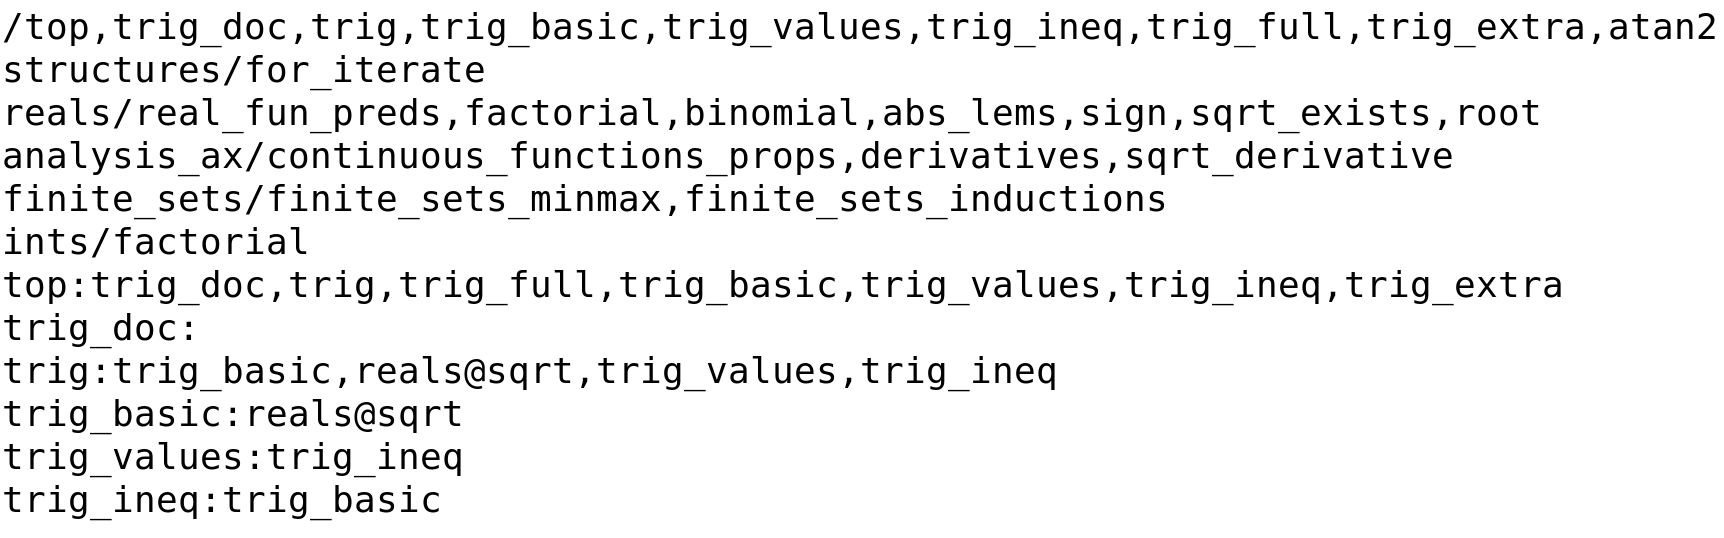
\includegraphics[width=11cm]{images/top.png}
  \caption{Overview of metadata file for package \cde{trig} in NASALib.}
  \label{fig.top}
\end{figure}


\section{Installation and Architecture}
\label{sec.install}

This section presents an overview of the installation procedure and
the distributed architecture of $\pvslm$.

The $\pvslm$ tool can be installed automatically from the command line
by issuing the following command:
%
\begin{verbatim}
  curl http://migueleci.github.io/pvslm/downloads/pvslm-conf.py \
    -o pvslm-install && chmod +x pvslm-install && \
    python ./pvslm-install
\end{verbatim}
%
This command uses the $\curl$ utility to download the $\pvslm$
installation sources from GitHub. Once these sources are downloaded
and some file permissions adjusted, the installation process is
executed as a Python 2 script. During the installation process, the
user can select the location in which the tool is to be installed,
including where the configuration files for the library sources and
the local copy of the libraries are to be placed. This script has been
tested both on Linux and Mac OS X boxes. Figure~\ref{fig.install}
depicts a successful installation procedure of $\pvslm$ in a Ubuntu
Linux box.

\begin{figure}
  \centering
  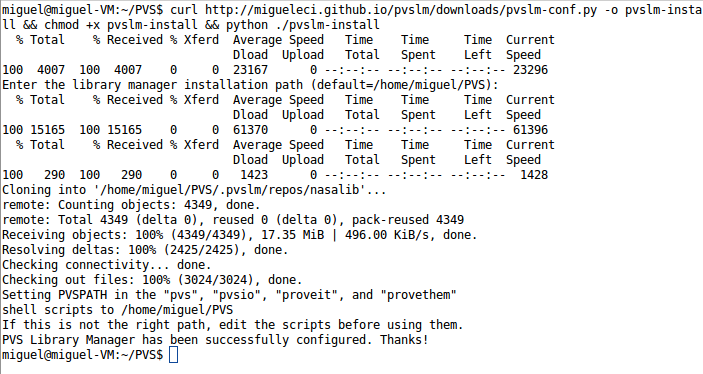
\includegraphics[width=11cm]{images/install.png}
  \caption{A successful installation procedure of $\pvslm$ in a Ubuntu
    Linux box.}
  \label{fig.install}
\end{figure}

Upon its successful installation, $\pvslm$ automatically configures
the NASALib library sources and makes a local copy of them by using
Git's clone command, so they are available for installation in PVS.

The $\pvslm$ tool is desiged with a distributed architecture. It can
connect to library sources over the internet. Each time a source is
configured, $\pvslm$ can download the library into the host system as
a local $\git$ repository. Further updates of the library are carried
out internally by $\pvslm$ by using $\git$'s pull
command. Figure~\ref{fig.arch} depicts the architecture of
$\pvslm$. It is important to note that although GitHub is used as
$\git$ server of reference throughout this paper, it is also possible
to use other publicly available servers such as BitBucket, for
instance, containing an annotated library.

\begin{figure}
  \centering 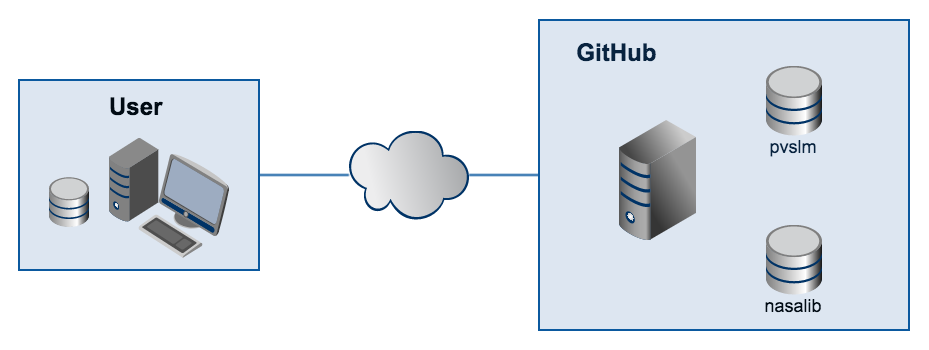
\includegraphics[width=11cm]{images/arch.png}
  \caption{Distributed architecture of $\pvslm$.}
  \label{fig.arch}
\end{figure}


\section{Case study: Managing NASALib with $\pvslm$}
\label{sec.nasalib}

This section presents a step-by-step guide on the configuration and
installation of the NASA PVS Library (NASALib) with the help of the
$\pvslm$ implementation. The current release of NASALib is annotated
with $\pvslm$'s description language and it is freely available from a
$\git$ repository in GitHub.

\paragraph{Library source creation.}
The first step is to issue a command for configuring the library sources
as follows:
%
{\small\begin{verbatim}
  $ pvslm.py src -a \\
      nasalib \\
      `The NASA PVS Library is a collection of formal PVS developments \\
         maintained by the NASA Langley Formal Methods Team.' \\
      https://github.com/nasa/pvslib.git
\end{verbatim}}
%
\noindent This command generates the library source configuration file
in the $\pvslm$ installation folder with the given information: a
library named \cde{nasalib}, with the given description, and whose
packages are available as a $\git$ repository from the given URL. At
this point, the configuration file is created but no packages are
downloaded nor installed from the repository. Note that it is not
possible to have two or more library sources with the same name.

It is important to note that this step is unnecessary with the current
distribution of $\pvslm$ because its installation script automatically
creates a library source configuration file for \cde{nasalib}. This
step is included for the sake of completeness of the example.

\paragraph{Downloading a library.} It is possible to use the $\pvslm$
implementation for downloading a library once its library source file
has been created. The following command downloads NASALib:
%
{\small\begin{verbatim}
  $ pvslm.py src -c nasalib
\end{verbatim}}
%
Internally, this command uses $\git$'s cloning technology so that the
NASALib repository is copied locally from the URL configured with the
library source.

\paragraph{Updating a library.} It is also possible to update a local
copy of a library. For updating the local copy of NASALib, an user can
issue the following command:
%
{\small\begin{verbatim}
  $ pvslm.py src -u nasalib
\end{verbatim}}
%
The effect of this command is to update the entire local copy of
\cde{nasalib} via $\git$'s pull command from the URL configured with
the library source.

\paragraph{Listing the contents of a library.} Once a local
copy of a library is available, it is possible to list all its
packages and their dependencies. The following command can be issued
to list the dependencies of package \cde{complex} in NASALib:
%
{\small\begin{verbatim}
  $ pvslm.py pkg -l nasalib@complex
\end{verbatim}}
%
The output of this command is as follows:
%
{\small\begin{verbatim}
  Package complex depends on:
  algebra
  analysis_ax
  ints
  lnexp
  reals
  structures
  trig
\end{verbatim}}

\paragraph{Installing a package in PVS.} The $\pvslm$ implementation
can install a package from a local copy of a library in a working PVS
environment. The following command installs package \cde{complex} from
NASALib:
%
{\small\begin{verbatim}
  $ pvslm.py pkg -i nasalib@complex
\end{verbatim}}
%
Since package \cde{complex} depends on other packages, the $\pvslm$
tool will ask for permission to install all these dependencies if they
are not already installed. The following is the output to the user for
this installation command.
%
{\small\begin{verbatim}
  Package complex depends on:
  ...
  Would you like to install the package(s) (y/N):
\end{verbatim}}
%
By convention, $\pvslm$ performs {\em all} installations in the folder
specified by the \cde{PVS\_PATH} global variable.

\paragraph{Deleting a package.} Finally, a user can issue the following
command to delete package \cde{ints} from the (internal) local copy of
NASALib:
%
{\small\begin{verbatim}
  $ pvslm.py pkg -d nasalib@ints
\end{verbatim}}
%
If there are packages that depend on the package to be removed, the
$\pvslm$ tool will list all of them and will ask the user for
authorization to also remove them.



% The very first letter is a 2 line initial drop letter followed
% by the rest of the first word in caps.
% 
% form to use if the first word consists of a single letter:
% \IEEEPARstart{A}{demo} file is ....
% 
% form to use if you need the single drop letter followed by
% normal text (unknown if ever used by the IEEE):
% \IEEEPARstart{A}{}demo file is ....
% 
% Some journals put the first two words in caps:
% \IEEEPARstart{T}{his demo} file is ....
% 
% Here we have the typical use of a "T" for an initial drop letter
% and "HIS" in caps to complete the first word.
%\IEEEPARstart{T}{his} demo file is intended to serve as a ``starter file''
%for IEEE Communications Society journal papers produced under \LaTeX\ using
%IEEEtran.cls version 1.8b and later.
% You must have at least 2 lines in the paragraph with the drop letter
% (should never be an issue)
%I wish you the best of success.

%\hfill mds
 
%\hfill August 26, 2015

%\subsection{Subsection Heading Here}
%Subsection text here.

% needed in second column of first page if using \IEEEpubid
%\IEEEpubidadjcol

%\subsubsection{Subsubsection Heading Here}
%Subsubsection text here.


% An example of a floating figure using the graphicx package.
% Note that \label must occur AFTER (or within) \caption.
% For figures, \caption should occur after the \includegraphics.
% Note that IEEEtran v1.7 and later has special internal code that
% is designed to preserve the operation of \label within \caption
% even when the captionsoff option is in effect. However, because
% of issues like this, it may be the safest practice to put all your
% \label just after \caption rather than within \caption{}.
%
% Reminder: the "draftcls" or "draftclsnofoot", not "draft", class
% option should be used if it is desired that the figures are to be
% displayed while in draft mode.
%
%\begin{figure}[!t]
%\centering
%\includegraphics[width=2.5in]{myfigure}
% where an .eps filename suffix will be assumed under latex, 
% and a .pdf suffix will be assumed for pdflatex; or what has been declared
% via \DeclareGraphicsExtensions.
%\caption{Simulation results for the network.}
%\label{fig_sim}
%\end{figure}

% Note that the IEEE typically puts floats only at the top, even when this
% results in a large percentage of a column being occupied by floats.


% An example of a double column floating figure using two subfigures.
% (The subfig.sty package must be loaded for this to work.)
% The subfigure \label commands are set within each subfloat command,
% and the \label for the overall figure must come after \caption.
% \hfil is used as a separator to get equal spacing.
% Watch out that the combined width of all the subfigures on a 
% line do not exceed the text width or a line break will occur.
%
%\begin{figure*}[!t]
%\centering
%\subfloat[Case I]{\includegraphics[width=2.5in]{box}%
%\label{fig_first_case}}
%\hfil
%\subfloat[Case II]{\includegraphics[width=2.5in]{box}%
%\label{fig_second_case}}
%\caption{Simulation results for the network.}
%\label{fig_sim}
%\end{figure*}
%
% Note that often IEEE papers with subfigures do not employ subfigure
% captions (using the optional argument to \subfloat[]), but instead will
% reference/describe all of them (a), (b), etc., within the main caption.
% Be aware that for subfig.sty to generate the (a), (b), etc., subfigure
% labels, the optional argument to \subfloat must be present. If a
% subcaption is not desired, just leave its contents blank,
% e.g., \subfloat[].


% An example of a floating table. Note that, for IEEE style tables, the
% \caption command should come BEFORE the table and, given that table
% captions serve much like titles, are usually capitalized except for words
% such as a, an, and, as, at, but, by, for, in, nor, of, on, or, the, to
% and up, which are usually not capitalized unless they are the first or
% last word of the caption. Table text will default to \footnotesize as
% the IEEE normally uses this smaller font for tables.
% The \label must come after \caption as always.
%
%\begin{table}[!t]
%% increase table row spacing, adjust to taste
%\renewcommand{\arraystretch}{1.3}
% if using array.sty, it might be a good idea to tweak the value of
% \extrarowheight as needed to properly center the text within the cells
%\caption{An Example of a Table}
%\label{table_example}
%\centering
%% Some packages, such as MDW tools, offer better commands for making tables
%% than the plain LaTeX2e tabular which is used here.
%\begin{tabular}{|c||c|}
%\hline
%One & Two\\
%\hline
%Three & Four\\
%\hline
%\end{tabular}
%\end{table}


% Note that the IEEE does not put floats in the very first column
% - or typically anywhere on the first page for that matter. Also,
% in-text middle ("here") positioning is typically not used, but it
% is allowed and encouraged for Computer Society conferences (but
% not Computer Society journals). Most IEEE journals/conferences use
% top floats exclusively. 
% Note that, LaTeX2e, unlike IEEE journals/conferences, places
% footnotes above bottom floats. This can be corrected via the
% \fnbelowfloat command of the stfloats package.

\section{Concluding Remarks}
\label{sec.concl}

This paper presented the $\pvslm$ tool for managing libraries for the
Prototype Verification System (PVS). This tool features support for
different library sources, libraries with several theories, and
dependencies among the theories (within the same library source).  The
tool is freely available for download and it is distributed under
GNU's GPLv3 license. It uses a small footprint language for
annotating libraries, which is described in full detail in BNF-like
notation in this paper. This paper also includes all commands
available from the tool, its architecture, and an overview of its
installation process.  A detailed step-by-step case study is included
for illustrating the main features of the tool.

As usual, much work remains to be done. First, it is important to make
available other PVS library sources with the help of the $\pvslm$
tool.  Also, it is important to test the tool against different
servers and in more operating systems. Finally, it would be highly
desirable for the tool to manage different versions of a library
source, each configured to work on different versions of PVS installed
in the host system. This will require an extension of the current
$\pvslm$ description language for annotating library sources.

\paragraph{\bf Acknowledgments.} The authors would like to thank
C. Mu\~noz in the NASA Langley Formal Methods Team for his
encouragement, ideas, and suggestions, specially for the help with the
definition of the metadata description language for packages.


% if have a single appendix:
%\appendix[Proof of the Zonklar Equations]
% or
%\appendix  % for no appendix heading
% do not use \section anymore after \appendix, only \section*
% is possibly needed

% use appendices with more than one appendix
% then use \section to start each appendix
% you must declare a \section before using any
% \subsection or using \label (\appendices by itself
% starts a section numbered zero.)
%


%\appendices
%\section{Proof of the First Zonklar Equation}
%Appendix one text goes here.

% you can choose not to have a title for an appendix
% if you want by leaving the argument blank
%\section{}
%Appendix two text goes here.


% use section* for acknowledgment
\section*{Acknowledgment}
The authors would like to thank
C. Mu\~noz in the NASA Langley Formal Methods Team for his
encouragement, ideas, and suggestions, specially for the help with the
definition of the metadata description language for packages.


% Can use something like this to put references on a page
% by themselves when using endfloat and the captionsoff option.
\ifCLASSOPTIONcaptionsoff
  \newpage
\fi



% trigger a \newpage just before the given reference
% number - used to balance the columns on the last page
% adjust value as needed - may need to be readjusted if
% the document is modified later
%\IEEEtriggeratref{8}
% The "triggered" command can be changed if desired:
%\IEEEtriggercmd{\enlargethispage{-5in}}

% references section

% can use a bibliography generated by BibTeX as a .bbl file
% BibTeX documentation can be easily obtained at:
% http://mirror.ctan.org/biblio/bibtex/contrib/doc/
% The IEEEtran BibTeX style support page is at:
% http://www.michaelshell.org/tex/ieeetran/bibtex/
%\bibliographystyle{IEEEtran}
% argument is your BibTeX string definitions and bibliography database(s)
%\bibliography{IEEEabrv,../bib/paper}
%
% <OR> manually copy in the resultant .bbl file
% set second argument of \begin to the number of references
% (used to reserve space for the reference number labels box)
%\begin{thebibliography}{1}
%\bibitem{IEEEhowto:kopka}
%H.~Kopka and P.~W. Daly, \emph{A Guide to \LaTeX}, 3rd~ed.\hskip 1em plus
%  0.5em minus 0.4em\relax Harlow, England: Addison-Wesley, 1999.
%\end{thebibliography}

\bibliographystyle{IEEEtran}
\bibliography{biblio}

% biography section
% 
% If you have an EPS/PDF photo (graphicx package needed) extra braces are
% needed around the contents of the optional argument to biography to prevent
% the LaTeX parser from getting confused when it sees the complicated
% \includegraphics command within an optional argument. (You could create
% your own custom macro containing the \includegraphics command to make things
% simpler here.)
%\begin{IEEEbiography}[{\includegraphics[width=1in,height=1.25in,clip,keepaspectratio]{mshell}}]{Michael Shell}
% or if you just want to reserve a space for a photo:

%\begin{IEEEbiography}{Michael Shell}
%Biography text here.
%\end{IEEEbiography}

% if you will not have a photo at all:
%\begin{IEEEbiographynophoto}{John Doe}
%Biography text here.
%\end{IEEEbiographynophoto}

% insert where needed to balance the two columns on the last page with
% biographies
%\newpage

%\begin{IEEEbiographynophoto}{Jane Doe}
%Biography text here.
%\end{IEEEbiographynophoto}

% You can push biographies down or up by placing
% a \vfill before or after them. The appropriate
% use of \vfill depends on what kind of text is
% on the last page and whether or not the columns
% are being equalized.

%\vfill

% Can be used to pull up biographies so that the bottom of the last one
% is flush with the other column.
%\enlargethispage{-5in}



% that's all folks
\end{document}


